\chapter{Architecture}

% \instructions{
%     Describe the architecture of your software as covered in the SEP2 module. The main goal of this chapter is describing the \textbf{technical implementation} in a way that a new team member can start working on the product as fast as possible.

%     \begin{itemize}
%         \item Use an existing template as a starting point (\texttt{arc42}, \texttt{C4 model}, ...)
%         \item Focus on stable, high-level concepts rather than details
%         \item Cover different views (static, dynamic, deployment, ...)
%         \item Prefer diagrams over text (ideally UML)
%         \item Explain the reasons behind your actions: \textit{Why did we build it like this?}
%     \end{itemize}
% }

Our application architecture is modelled using the C4 model combined with Clean Architecture. We decided to use two levels of the C4 model, because it gives a good overview how the different components of our application talk with each other and other systems. We replaced the remaining levels of the C4 model with Clean Architecture, because it is a better representation of how our source code dependencies are structured.
Our application is built to use metrics which are scraped and stored by Prometheus from a Kubernetes cluster.
The functional requirements FR1 to FR11 that are tracked on GitLab have been reviewed and can all be satisfied with this architecture.
The non-functional requirements NFR-2, NFR-3, NFR-4, are possible to satisfy with the technologies shown in the section Clean Architecture.
The application will be built inside a container to satisfy NFR-5.

\section{Roles}
The role of the architect is split up. We work according to the architecture agent model, where we have two architects.
Jan is responsible for Kubernetes, Prometheus, CI/CD, i.e. the architecture at large
and Pascal is responsible for the architecture of our web application, which libraries are used and how we connect the different components, i.e. the "architecture in detail". We decided to use the model with two main architects, because the project can be easily split into two parts the Web application itself and interfacing systems. So there is one person from each part to discuss the interfaces between the two parts to get the perfect architecture over all.

\section{System Architecture according to C4 model}
\begin{figure}[H]
  \centering
  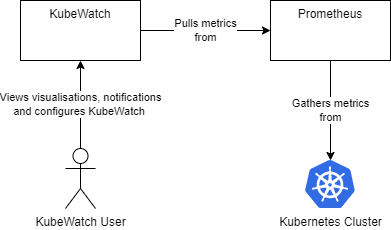
\includegraphics[height=5cm]{resources/System_context_diagram.png}
  \caption{System context diagram}
  \label{fig:system-context-diagram}
\end{figure}

\begin{figure}[H]
  \centering
  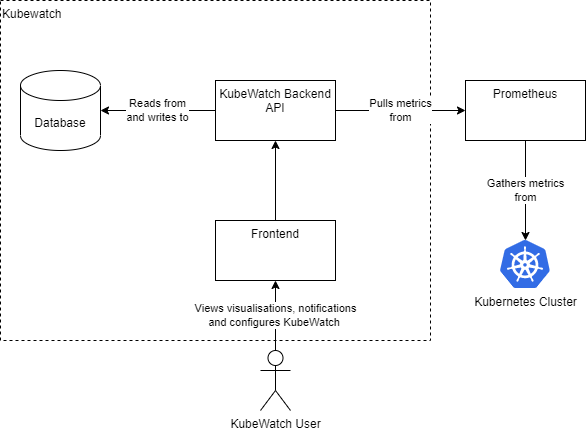
\includegraphics[height=8cm]{resources/Container_diagram.png}
  \caption{Container diagram}
  \label{fig:container-diagram}
\end{figure}

\pagebreak
\section{CI/CD Pipeline Architecture}
At each push from our project to the gitlab environment, the CI/CD pipeline runs and starts different jobs, depending on the changed files.

Our pipeline consists of three stages: \textit{build, test, deploy}. Each of these stages is described in more detail in the following section.

\subsection{Pipeline Stages}
\textbf{Build:} This stage is used to build the documentation pdf file. It is also used to build the docker image which is used to publish our application container image in the gitlab container registry which is needed by the deployment stage to deploy our application to the cluster.


\textbf{Test:} This stage is used to test our application. We automated as many tests as possible to minimize the effort on the team needed for testing. The advantage of this, is that tests can not be get forgotten. We can perform all \textit{Unit Tests} and \textit{Integration Tests} within this test stage of the ci/cd pipeline.


\textbf{Deploy:} In our last pipeline stage, we deploy the newest version of our application to the Kubernetes cluster located inside the INS network, to be able to present the current main version of the application.

\subsection{Accessing Deployed Application}
To access current main version of KubeWatch, you need to be connected to the INS network via VPN. Then you can find the web application deployment in Gitlab in the \href{https://gitlab.ost.ch/SEProj/2022-FS/g03-kubewatch/kubewatch/-/environments}{Deployments / Environments} section and there you can \textit{Open} the web application.

\begin{figure}[H]
  \centering
  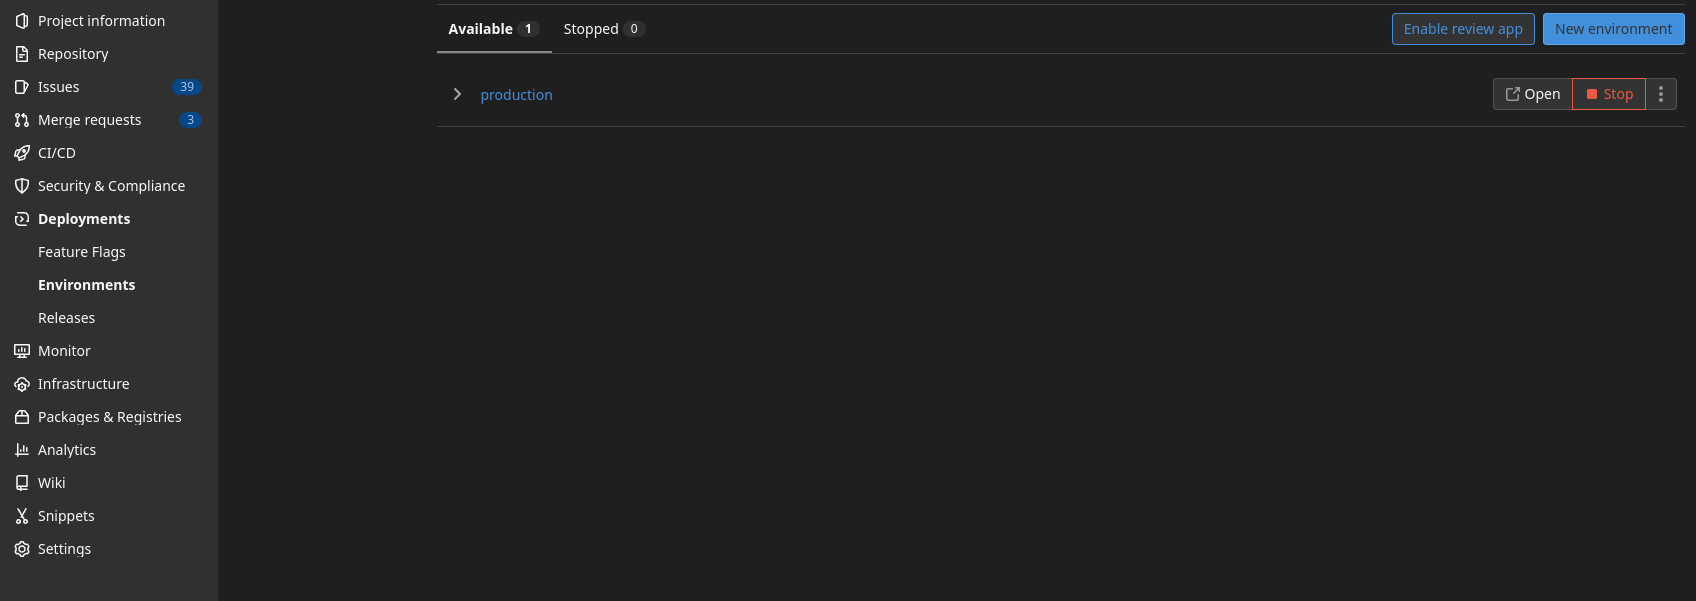
\includegraphics[width=\textwidth]{resources/web-application-INS.png}
..\label{fig:deployment-environment}
\end{figure}

\section{Web App Clean Architecture}
\begin{figure}[H]
  \centering
  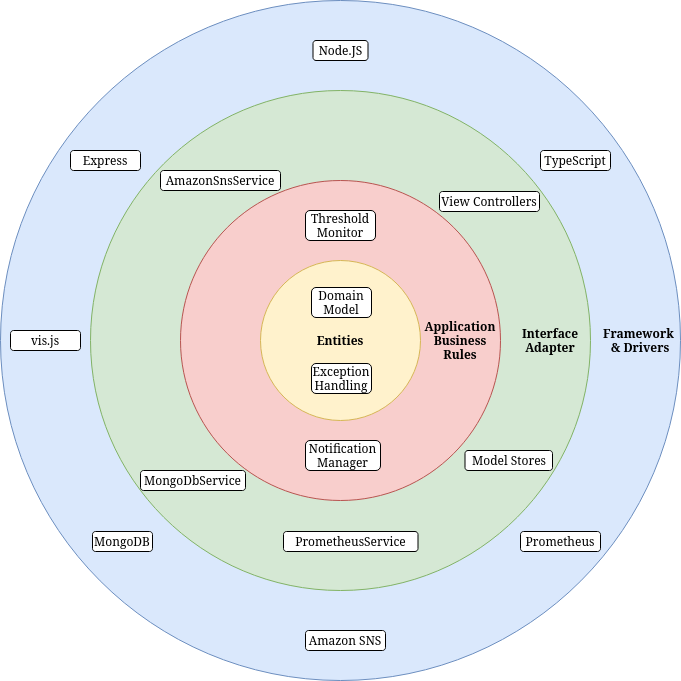
\includegraphics[height=14cm]{resources/clean_architecture.drawio.png}
  \caption{Web app clean architecture}
  \label{fig:web-app-architecture}
\end{figure}

\begin{table}[H]
  \begin{tabular*}{\textwidth}{p{3cm} | p{11cm}}
    \textbf{Entities:} &
      These are components shared by the whole system and are contained
      in the \textit{/model} directory.
      This includes the classes from the domain model and the model store interfaces,
      allowing implementation from the Interface Adapter layer. \bigskip \\
    \textbf{Application Business Rules:} &
      This layer contains our business logic and is contained in
      the \textit{/domain} directory. \bigskip \\
    \textbf{Interface Adapter:} &
      This is the place for logic to attach to our external dependencies
      like Prometheus and MongoDB and is contained in the \textit{/services} directory.
      The \textit{/view-controllers} directory contains the code
      that prepares the data to be displayed on the website.
      And the implementations of the model store interfaces are stored
      in the \textit{/stores} directory. \bigskip \\
    \textbf{Framework \& Drivers:} &
      These are the major frameworks and dependencies powering our application. \\
  \end{tabular*}
  \caption{Clean-Architecture layers explained}
  \label{tab:clean-architecture-layers-explained}
\end{table}

\subsection{Scaling}

State that should persist through a web page refresh, should be stored using a interface adapter for persistence. This allows the application in combination with our \hyperref[section:non-functional-requirements]{NFR Section} to be horizontally scaleable.

\section{Wireframe}

To visualise the application draft we decide to use a wireframe because it makes a lot of sense with the web application \textit{KubeWatch} we programme in this project. So for a detailed overview, we can just click through the wireframe to get an impression. The complete wireframe can be found as a PDF\footnote{\url{https://gitlab.ost.ch/SEProj/2022-FS/g03-kubewatch/kubewatch/-/blob/main/Documentation/appendix/wireframe_kubewatch.drawio.pdf}} and HTML page\footnote{\url{https://gitlab.ost.ch/SEProj/2022-FS/g03-kubewatch/kubewatch/-/blob/main/Documentation/appendix/wireframe_kubewatch.drawio.html}} in the appendix directory.
The HTML page is interactive.

\section{Class Diagram}
The current class diagram can be easily generated with \textit{Webstorm} and is placed in the appendix folder\footnote{\url{https://gitlab.ost.ch/SEProj/2022-FS/g03-kubewatch/kubewatch/-/blob/main/Documentation/appendix/class_diagram_from_webstorm.png}}.
For this select the relevant folders with the mouse.
Right-click on it and select \textit{Diagrams} \textrightarrow \textit{Show Diagram}.
